\documentclass[tikz,border=10pt]{standalone}
\usetikzlibrary{arrows.meta, positioning, shapes.geometric, fit}

\begin{document}
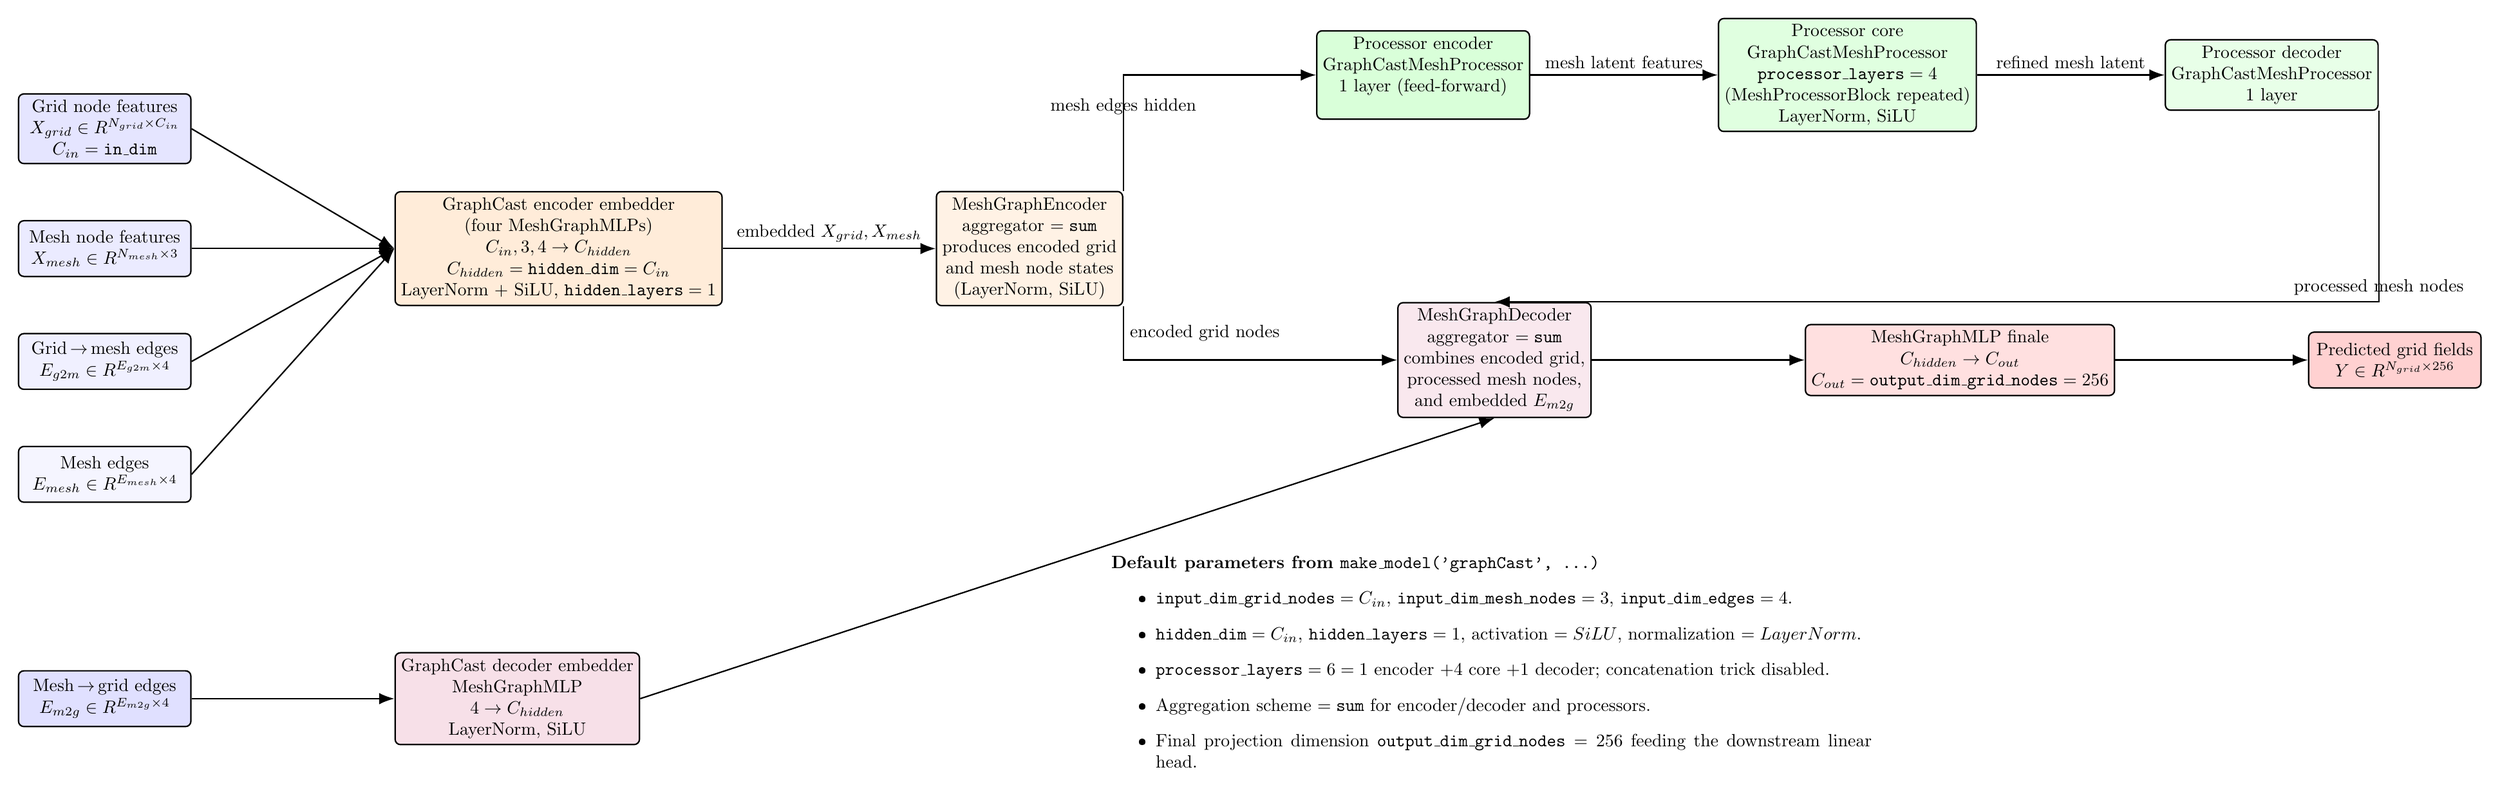
\begin{tikzpicture}[
    block/.style={draw, thick, minimum width=3.4cm, minimum height=1.3cm, align=center, rounded corners=3pt},
    data/.style={draw, thick, minimum width=3.4cm, minimum height=1.1cm, align=center, rounded corners=3pt, fill=blue!10},
    arrow/.style={-{Latex[length=3mm]}, thick},
    node distance=1.5cm
]
    % Inputs
    \node[data] (gridin) {Grid node features\\$X_{\text{grid}} \in \mathbb{R}^{N_{\text{grid}} \times C_{\text{in}}}$\\$C_{\text{in}} = \texttt{in\_dim}$};
    \node[data, below=1.1cm of gridin, fill=blue!8] (meshin) {Mesh node features\\$X_{\text{mesh}} \in \mathbb{R}^{N_{\text{mesh}} \times 3}$};
    \node[data, below=1.1cm of meshin, fill=blue!6] (g2min) {Grid\,$\rightarrow$\,mesh edges\\$E_{g2m} \in \mathbb{R}^{E_{g2m} \times 4}$};
    \node[data, below=1.1cm of g2min, fill=blue!4] (meshedgein) {Mesh edges\\$E_{\text{mesh}} \in \mathbb{R}^{E_{\text{mesh}} \times 4}$};

    % Encoder embedder
    \node[block, right=4.0cm of meshin, fill=orange!15] (embedder) {GraphCast encoder embedder\\(four MeshGraphMLPs)\\$C_{\text{in}},3,4 \rightarrow C_{\text{hidden}}$\\$C_{\text{hidden}} = \texttt{hidden\_dim} = C_{\text{in}}$\\LayerNorm + SiLU, $\texttt{hidden\_layers} = 1$};

    \draw[arrow] (gridin.east) -- (embedder.west);
    \draw[arrow] (meshin.east) -- (embedder.west);
    \draw[arrow] (g2min.east) -- (embedder.west);
    \draw[arrow] (meshedgein.east) -- (embedder.west);

    % Mesh graph encoder
    \node[block, right=4.2cm of embedder, fill=orange!10] (encoder) {MeshGraphEncoder\\aggregator $= \texttt{sum}$\\produces encoded grid \\and mesh node states\\(LayerNorm, SiLU)};

    \draw[arrow] (embedder) -- node[above]{embedded $X_{\text{grid}}, X_{\text{mesh}}$} (encoder);

    % Processor blocks
    \node[block, above right=1.4cm and 3.8cm of encoder, fill=green!15] (procenc) {Processor encoder\\GraphCastMeshProcessor\\1 layer (feed-forward)\\};
    \node[block, right=3.7cm of procenc, fill=green!12] (proccore) {Processor core\\GraphCastMeshProcessor\\$\texttt{processor\_layers} = 4$\\(MeshProcessorBlock repeated)\\LayerNorm, SiLU};
    \node[block, right=1.4cm and 3.7cm of proccore, fill=green!9] (procdec) {Processor decoder\\GraphCastMeshProcessor\\1 layer};

    \draw[arrow] (encoder.north east) |- node[pos=0.3, above]{mesh edges hidden} (procenc.west);
    \draw[arrow] (procenc) -- node[above]{mesh latent features} (proccore);
    \draw[arrow] (proccore) -- node[above]{refined mesh latent} (procdec);
    
    % Decoder embedder input
    \node[data, below=3.3cm of meshedgein, fill=blue!12] (m2gin) {Mesh\,$\rightarrow$\,grid edges\\$E_{m2g} \in \mathbb{R}^{E_{m2g} \times 4}$};
    \node[block, right=4.0cm of m2gin, fill=purple!12] (decembed) {GraphCast decoder embedder\\MeshGraphMLP\\$4 \rightarrow C_{\text{hidden}}$\\LayerNorm, SiLU};
    \draw[arrow] (m2gin.east) -- (decembed.west);

    % MeshGraphDecoder
    \node[block, right=5.4cm of encoder, yshift=-2.2cm, fill=purple!9] (decoder) {MeshGraphDecoder\\aggregator $= \texttt{sum}$\\combines encoded grid,\\processed mesh nodes,\\and embedded $E_{m2g}$};

    \draw[arrow] (encoder.south east) |- node[pos=0.25, right]{encoded grid nodes} (decoder.west);
    \draw[arrow] (procdec.south east) |- node[pos=0.5, above]{processed mesh nodes} (decoder.north);
    \draw[arrow] (decembed.east) -- (decoder.south);

    % Finale MLP
    \node[block, right=4.2cm of decoder, fill=red!12] (finale) {MeshGraphMLP finale\\$C_{\text{hidden}} \rightarrow C_{\text{out}}$\\$C_{\text{out}} = \texttt{output\_dim\_grid\_nodes} = 256$};
    \draw[arrow] (decoder) -- (finale);

    \node[data, right=3.8cm of finale, fill=red!18] (gridout) {Predicted grid fields\\$Y \in \mathbb{R}^{N_{\text{grid}} \times 256}$};
    \draw[arrow] (finale) -- (gridout);

    % Legend
    \node[below=2.6cm of decoder, align=left] (legend) {
        \begin{minipage}{15cm}
            \textbf{Default parameters from \texttt{make\_model('graphCast', \dots)}}
            \begin{itemize}
                \item $\texttt{input\_dim\_grid\_nodes} = C_{\text{in}}$, $\texttt{input\_dim\_mesh\_nodes} = 3$, $\texttt{input\_dim\_edges} = 4$.
                \item $\texttt{hidden\_dim} = C_{\text{in}}$, $\texttt{hidden\_layers} = 1$, activation $= \text{SiLU}$, normalization $= \text{LayerNorm}$.
                \item $\texttt{processor\_layers} = 6 = 1$ encoder $+ 4$ core $+ 1$ decoder; concatenation trick disabled.
                \item Aggregation scheme $= \texttt{sum}$ for encoder/decoder and processors.
                \item Final projection dimension $\texttt{output\_dim\_grid\_nodes} = 256$ feeding the downstream linear head.
            \end{itemize}
        \end{minipage}
    };

\end{tikzpicture}
\end{document}
